\chapter{Methodology and data Gathering}
\label{chapter:methodology}
This thesis will be focused mainly on classification problem of the "human presence" i.e. if the human is present or not. This will be a supervised learning problem where the features will be mapped to the classes/labels.
For this thesis, we are using VTT built 25 GHz radar.The methodology includes Data collection, Data cleaning, Model Building and Model deployment. Here is a flow, how the process will be conducted in the upcoming months.


\begin{figure}[ht]
  \begin{center}
    % below the size of the figure has been reduced for example
    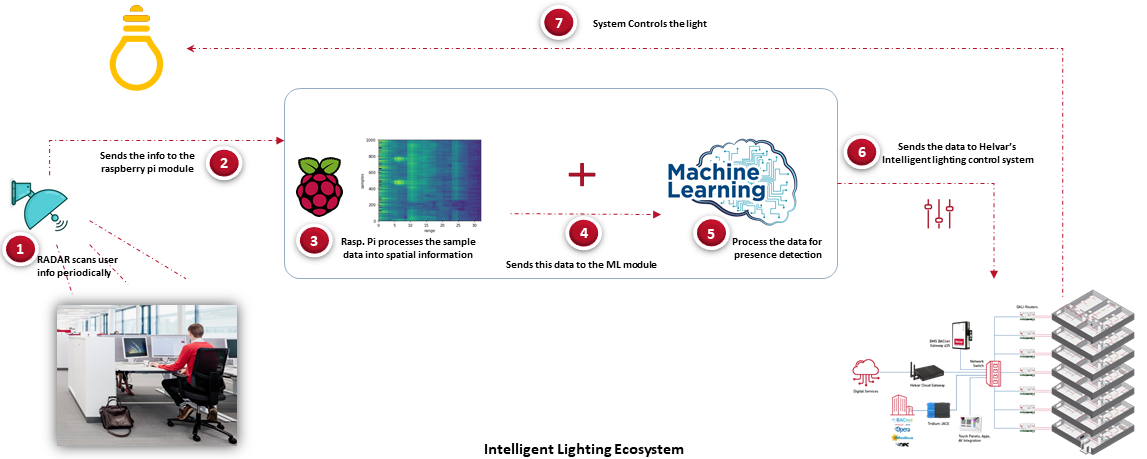
\includegraphics[width=1\textwidth]{Master's thesis/images/thesis_presentation.png} 
    \caption{Overall Process}
    \label{fig:basic_principle}
  \end{center}
\end{figure}


\begin{enumerate}
    \item RADAR box provides Analog to Digital converted signal. The data from these signals are collected over multiple hours at multiple locations.
    %However, this information is not sufficient to distinguish between human presence or absence. Therefore, in order to detect human presence i.e. to collect the labels for the data, we will be using RGB camera for the purpose of creating ground truth. Radar data will be mapped with RGB presence detection based on each time frame.
    \item The data obtained will be feature engineered using multiple techniques.
    \item The idea is to engineer the received radar signal of every time frame (say 1 sec) to a 2-D map and then treating this 2-D map as an image or set of features.
    \item Deep Neural Networks or other Machine Learning techniques will be applied on this already processed data.
    \item For the purpose of training, we will leverage the cloud resources by AWS.
    \item The last step is to deploy these models on the edge devices.
\end{enumerate}

The ultimate objective is to create a more sustainable lighting control solution. Currently at Helvar, the most effective control system turns off the luminaires after 10 min of human absence. Even if, we are able to bring down these power wasteful windows by 50 \%, it would make huge impact on the society. Not only it will contribute to sustainability but will also result in lower power consumption and therefore less electricity bills. Lastly, it will add a lot of business value to Helvar as a company. In the following sections, we shall discuss the steps specified above in thorough detail.

\section{Experimental Design and Setup}

\subsection{Data Collection with Radar}
RADAR itself cannot be used for direct communication with a workstation. That is why, Raspberry Pi 4 is used for communication. Raspberry Pi 4 acts as a mediator between the RADAR and a workstation through which data is being processed or analysed. 
The Radar is connected to Raspberry Pi 4 internally and packed inside a 3D printed case, thus forming one module. Please be aware in further discussions, we will be referring this box i.e combination of RADAR and Raspberry Pi 4 as RADAR Box or just RADAR for the purpose of simplicity. When supplied power, the Raspberry Pi 4 inside the box opens a hot-spot for secure connection.The RADAR Box is then connected to the workstation using SSH. 

\begin{figure}[ht]
  \begin{center}
    % below the size of the figure has been reduced for example
    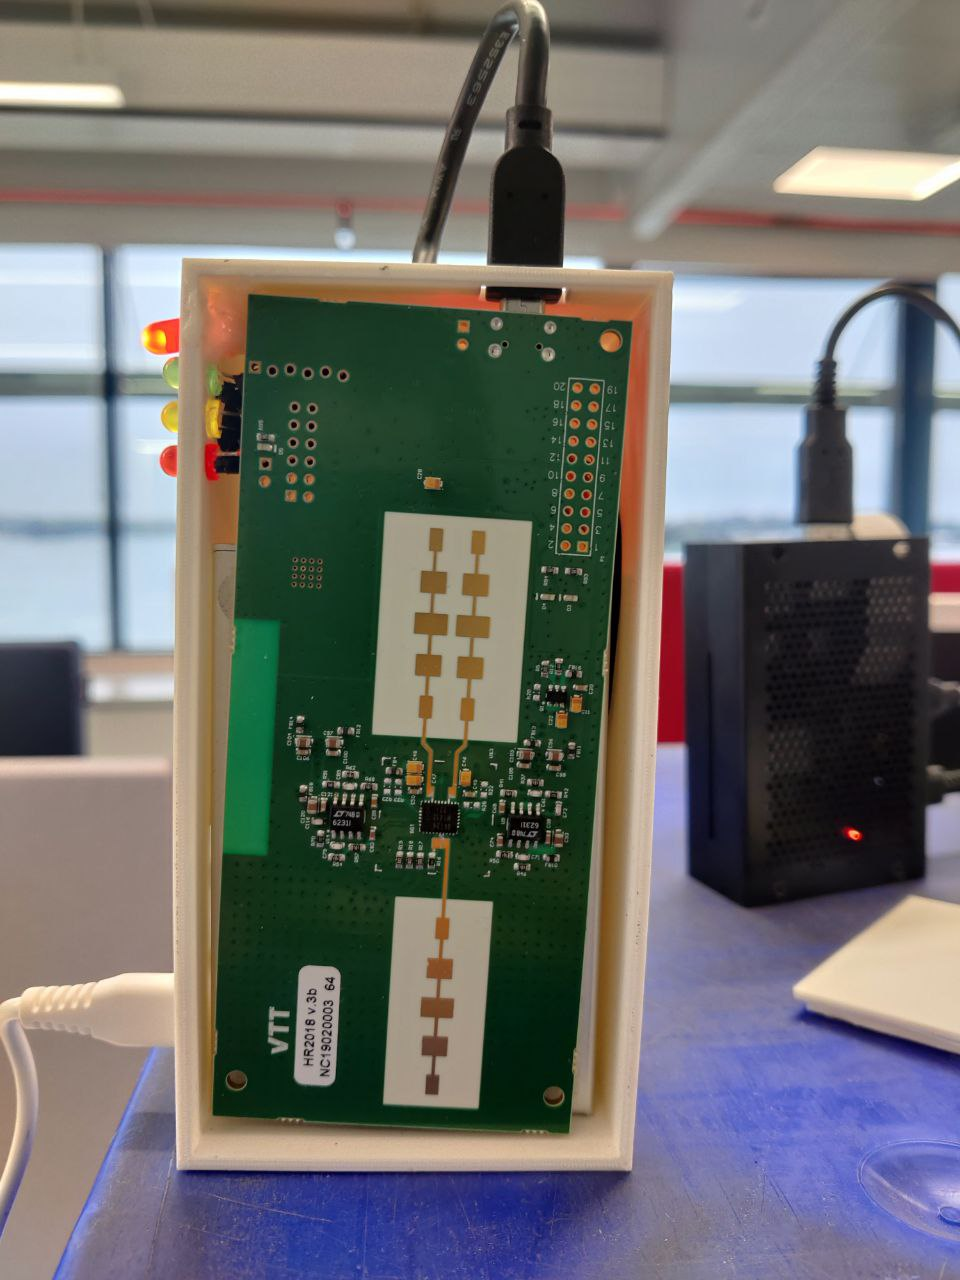
\includegraphics[width=0.5\textwidth]{Master's thesis/images/radar_int.jpg} 
    \caption{The Radar Box - RADAR + Raspberry Pi4 }
    \label{fig:AoA}
  \end{center}
\end{figure}  

The program inside the Rpi to read data from RADAR is executed via this SSH. In order to send data from Rpi to the workstation, MQTT is used. The Message Queuing Telemetry Transport (MQTT) is a lightweight, publish-subscribe network protocol that transports messages between devices.It is designed for connections with remote locations where a "small code footprint" is required or the network bandwidth is limited ~\cite{wikipedia_mqtt}.  The hierarchy includes one broker and multiple clients. The broker receives all the messages from all the clients and then forwards to appropriate destinations. Information is organized in the form of topics. When a client publishes information on Topic A to broker, the broker sends this information to all the clients who have subscribed to this topic.

RADAR Box publishes information to a broker, and then broker sends the information to the workstation. The information received by the workstation is the actual received signals of the received antenna of the RADAR.  Instead of using a local workstation for storing the data, AWS S3 buckets are used for storing the data. AWS S3 is efficient method of storing as high volumes of data that can be easily accessed by people having the authorization.


%Data packet ( combination of chirps)
To dump the data to AWS, an efficient packaging technique for data was required. One Antenna of the RADAR generates 497 samples, i.e, 2x497 samples per chirp for two receiver antennas. In the basic raw mode, the time difference between two consecutive chirps is 31.25 ms. This means ,RADAR generates 2x497 samples in 31.25 ms or 32x2x497 samples in 1 sec. 
One way is to treat the signals of 1 chirp as one datum i.e one data sample with 2x497 feature vectors, however there is  a problem with this approach. For an instance time associated with this data is very less and features per chirp are not sufficient enough for our deep learning model to make an efficient prediction. Therefore, multiple chirps are stacked together to form one datum. In this thesis 32 chirps are stacked together to obtained one datum which represents 1 sec of signals. This approach will even make the labelling much easier which is explained in a more elaborate manner in the next section.

So in summary, the data produced every second is stacked together in the file format and then dumped to AWS S3 buckets.It is worth mentioning that the name of the file is the timestamp at which the first chirp was transmitted. This helps in storing the data properly and it makes it really simple to compare the data with an RGB camera, which will be explained in the next section.


\subsection{Ground truth with RGB camera}
\label{section:environments}
The Radar is set to receive signals for the time span of 31.25 ms. This means in one second, an approximate of 32 signals are generated. The RADAR data is collected for multiple days in a meeting room of Helvar's headquarters in Espoo. This means on average, the radar generated 32x60x60x24 samples in 1 day. In an ever-moving environment like IT offices, its almost impossible to annotate such vast amount of data manually. It's not possible to label if a person was present or not for every second for the radar data manually.  One approach was to label the data using the meeting calendars i.e. label the data True if the meeting room is booked. But this approach is highly prone to false labelling. For an example, a meeting room can be occupied by a person even if its not booked. On the other hand, it may be possible that no one comes to the meeting the meeting room despite the booking. Therefore, the more reliable labelling mechanism was desired.

The other way to do was to record a video of the same at the same time of the RADAR and then using this video to annotate the data manually. This approach is again prone to a lot of loopholes, for e.g manual annotation for days and days of data require a lot of extra effort. Apart from effort, this manual annotation method is really not scalable when we are dealing with commercial usage. It works fine for research based, but in an industry when eventually clients are involved, there is a need for exploring a better automatic solution. 

The data which is used in this thesis is hours and hours of data. In order to achieve reliable inference from our data, precise labelling is required for the training set. Therefore, for creating the labels for the Radar data for training set, an RGB camera is used. Raspberry Pi 8.0 Mpix v2 camera is used for this thesis, has a Sony IMX219 8-megapixel sensor. The Camera Module can be used to take stills photographs as well as high-definition video. It supports 1080p30, 720p60 and VGA90 video modes, as well as still capture. The module is attached via a 15cm ribbon cable to the CSI port on the Raspberry Pi ~\cite{raspberrypi}.
\begin{figure}[ht]
  \begin{center}
    % below the size of the figure has been reduced for example
    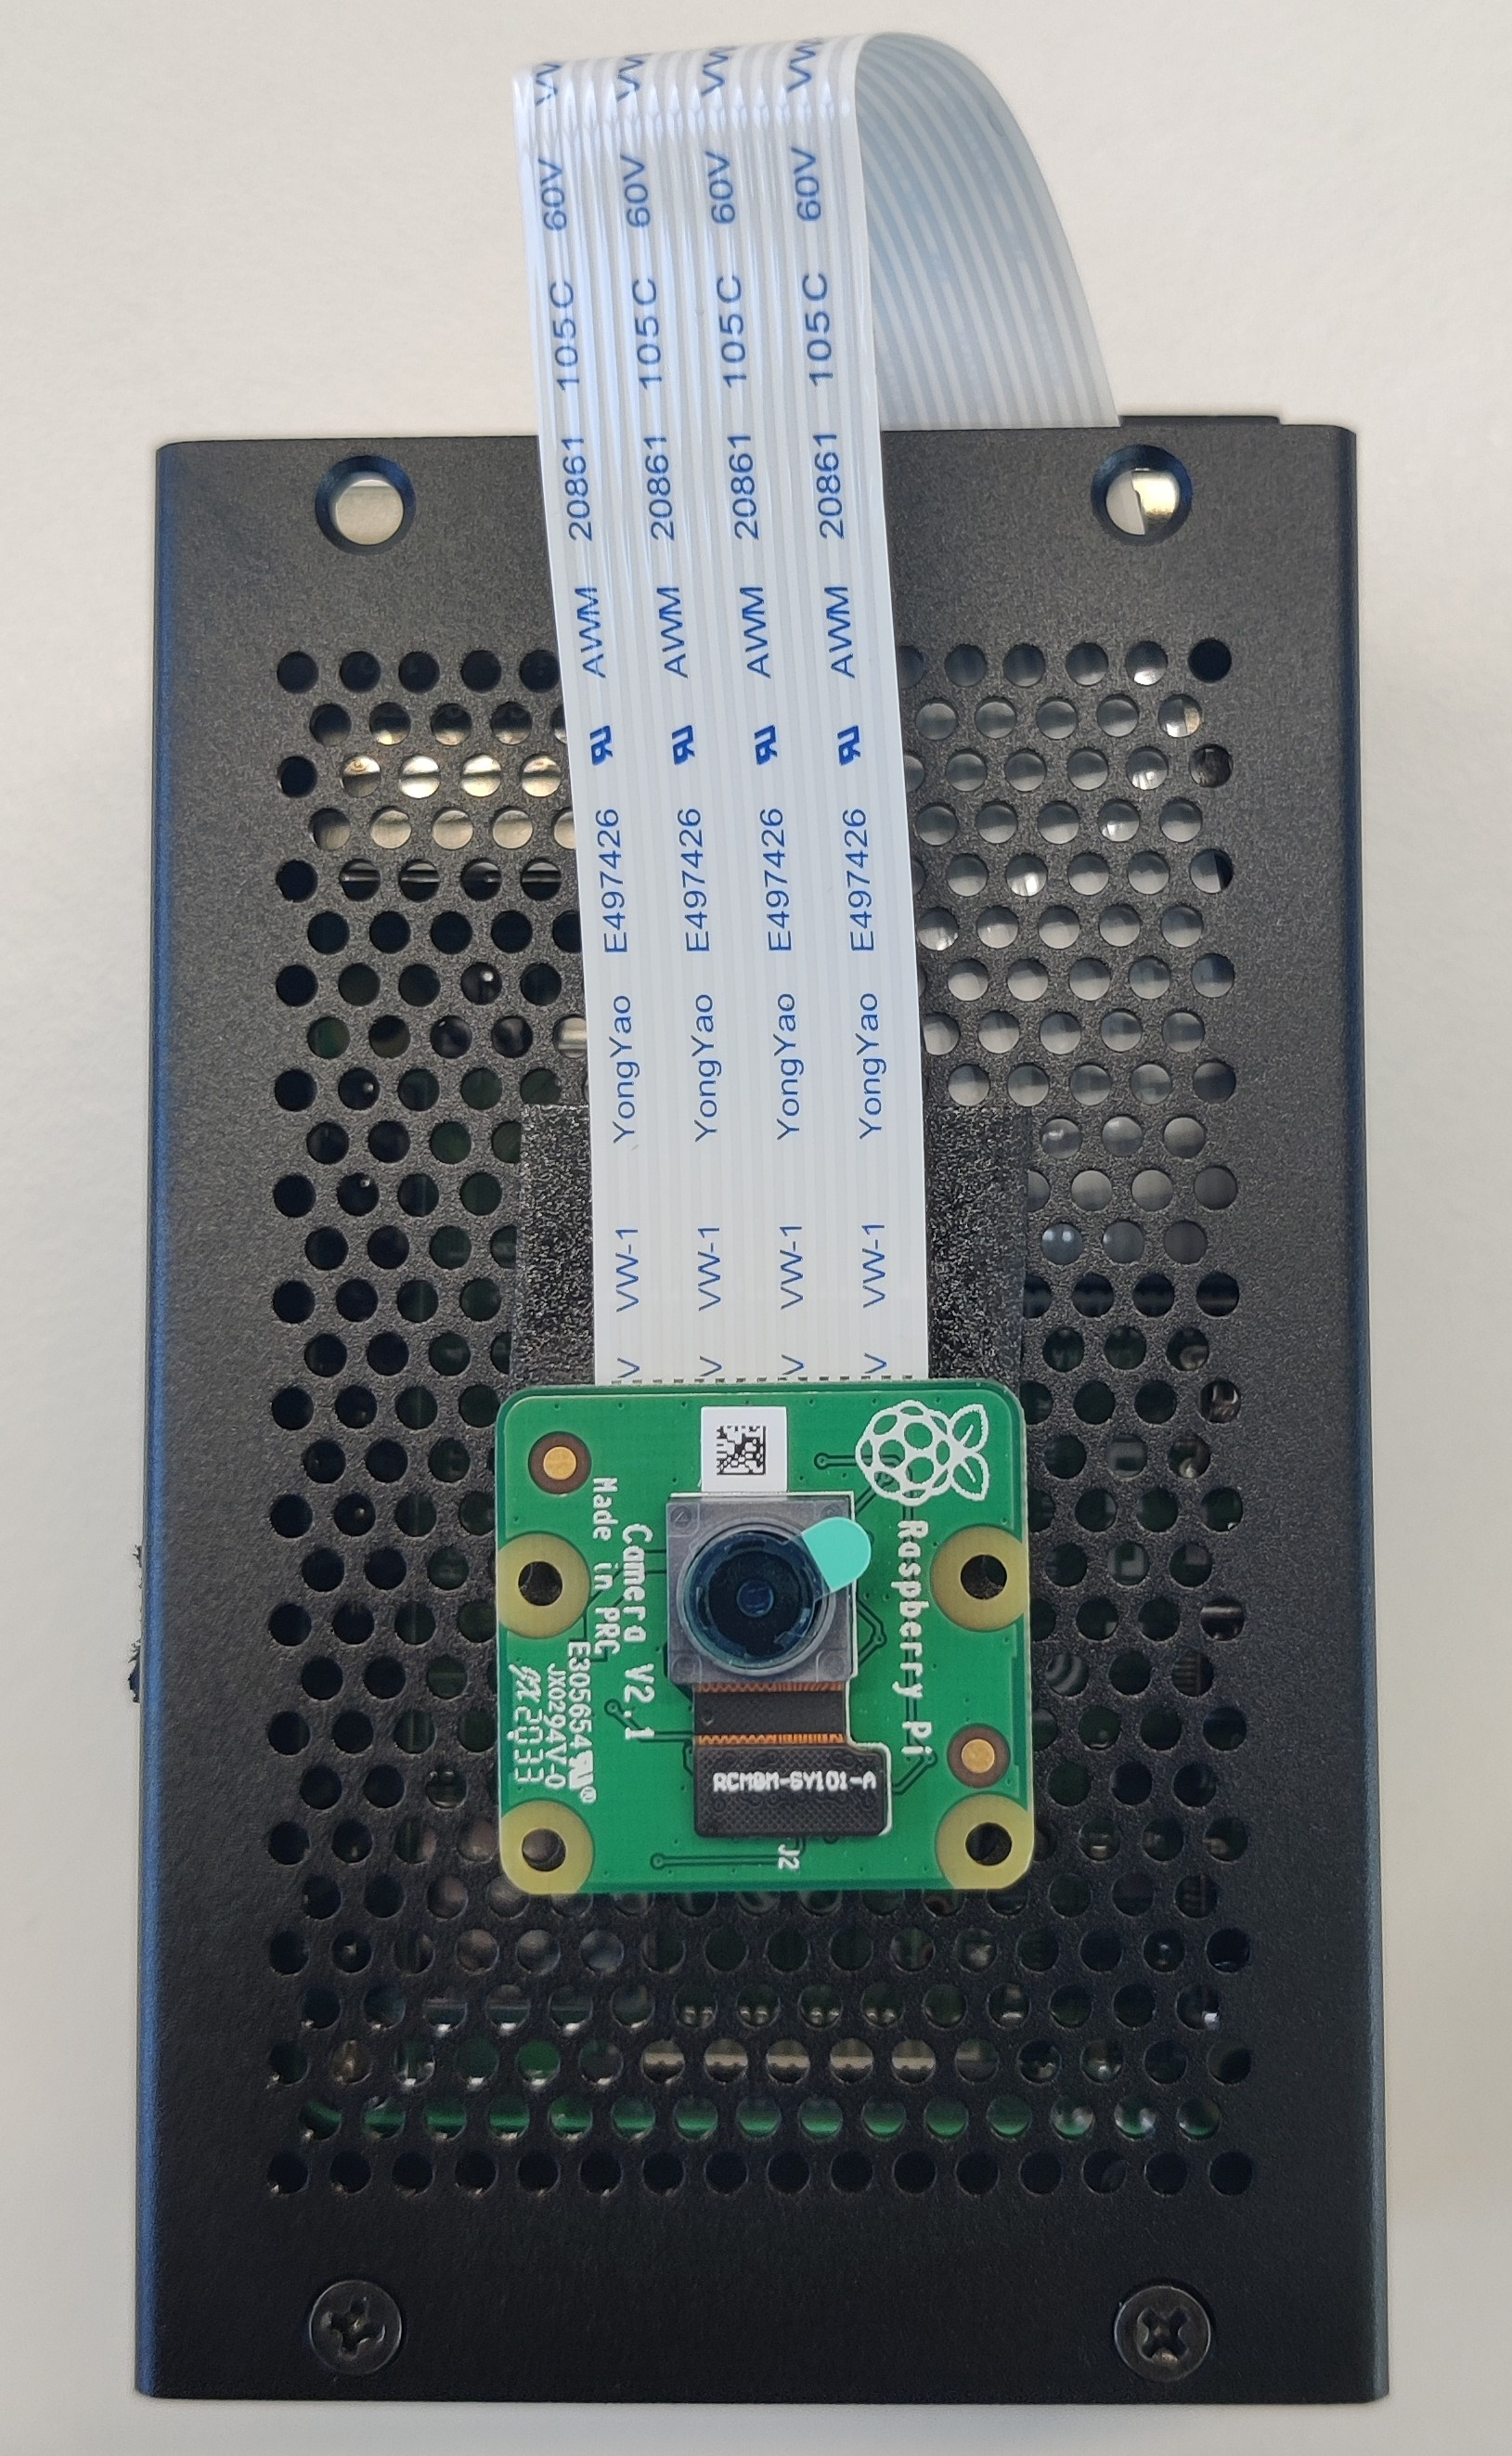
\includegraphics[scale = 0.07]{Master's thesis/images/RGB_camera.jpg} 
    \caption{The RGB Camera}
    \label{fig:AoA}
  \end{center}
\end{figure}  
However, instead of manually annotating these videos, the use cases of Machine Learning and Deep Learning are leveraged. With the advancement of Machine Learning and Deep Learning libraries, object detection and object recognition can be done with accuracy as high as 100 \%. This field of artificial intelligence that trains computers to interpret and understand the visual world is called Computer Vision. With the advancement of AI and innovations in deep learning and neural networks, Computer Vision been able to take great leaps currently and has been able to surpass humans intelligence in some tasks related to detecting and labeling objects for optical sensors.


The RGB camera in the experiment and Radar are mounted next to each other, so that the field of view of Radar and camera overlaps. The camera used in this thesis captures 60 frames per second (fps). For the purpose of labelling the Radar data, the scene is captured with an RGB camera alongside Radar. The camera is connected to a 32-bit Raspberry pi 4. This Rpi leverages the camera to record videos. Each video file spans 1 second. The name of the file is the timestamp at which the file was created. As soon as the file is created, a parallel process dumps the data periodically to the AWS bucket. In order to prevent Rpi from memory overload, the files from the Rpi are removed as soon as they are dumped to AWS successfully.. The important thing to notice here is the duration of the video. 1 sec is chosen so that it is easy later on to combine RADAR data as well RGB data later on.Once the data is dumped, the data is cleaned For an instance, the videos of size 0 Kb are removed. These are the lost packets or the unsuccessful video captures.

\subsection{Platform for collecting Data}
For this thesis, Data collected is huge. It is almost impossible for a local machine to run heavy computations on such a high volume of data. Therefore in order to run heavy computations without any memory leaks, the best possible technology available is the use of Cloud Resources. For the purpose of this thesis, we are using AWS EC2 instances. AWS EC2 instances are fast reliable and will be able to access the S3 buckets directly. 

There are different parameters to be taken into account while deciding to use CPU's or GPU's to train the deep learning models. Those parameters include the memory bandwidth, GPU has on average better memory bandwidth in comparison to CPU's. Considering the data-set size, the larger the data-set the more advantage the GPU will have over CPU. As for the Parallelism of the model, some models have more parallelism than others. For example, Fast Forward Neural Networks 8 FNN's) and Convlutional Neural Networks (CNN's) can support high parallelism, therefore, it can be applied better on a Single Instruction Multiple Data (SIMD) processor such as the GPUs. Finally, coming to Cost-effectiveness, the power cost of GPU is higher than the CPU. For non parallel processes or less parallel processes like Recurrent Neural Networks, it is better to use a CPU. In this work, the cloud instances based on CPU or GPU is used to train the models according to the needs as mentioned above.

For this thesis, Deep Learning Base AMI Ubuntu instance is used of type p2.xlarge is used. Deep learning instance is launched in order to use the GPU instances for running the Deep Learning models.P2 instances provide up to 16 NVIDIA K80 GPUs, 64 vCPUs and 732 GiB of host memory, with a combined 192 GB of GPU memory, 40 thousand parallel processing cores, 70 teraflops of single precision floating point performance, and over 23 teraflops of double precision floating point performance ~\cite{amazonec2}. 


\subsection{Computing on Cloud for RGB Data}

The data collected from RGB data which is stored in S3 buckets can be directly accessed from EC2 instance as both the instance and the bucket are present in the same AWS region.  For this project a hybrid of  two techniques are used for object detection on the RGB data collected. 
\begin{enumerate}
    \item \textbf{YOLOv3} - YOLOv3 is chosen because it is extremely fast and accurate. The mAP of YOLOv3 is measured at .5 IOU  which is is on par with Focal Loss but about 4x faster. YOLOv3 uses a few tricks to improve training and increase performance, including multi-scale predictions, a better backbone classifier, and more ~\cite{yolo_time}. YOLOv3 returns output in the form of pre defined 80 classes on which the model is trained. Here in this thesis, only person class is a matter of interest. In order to detect only human, the detection class of the YOLOv3 model has been manipulated.
    \item \textbf{Motion Detection} - This technique is used to detect motion in a scene. It is used because sometimes it is possible for a person to be occluded in the video. For an instance, consider a person half occluded behind the desktop monitor, or a scenario where there is only hand moving in front of camera, or where someone is half visible behind the door, for such scenarios YOLOv3 will fail because there are a lot of occlusions present in the same. Therefore for such cases, motion detection algorithm is used on the RGB camera data. When the movement is beyond a fix threshold, only then the algorithm returns presence, otherwise it ignores small movements, for e.g., movement due to curtains or leaves of the plants are ignored. The approach is very simple and self intuitive. When the program starts, it will capture a called baseline image. The program will keep comparing the new frame with this baseline image. If there is a movement in the new frame, the contents of the image will be different and if this difference is beyond a certain threshold,  the program will return Presence.
\end{enumerate}

Once the data is cleaned into AWS, YOLOv3 and  Motion Detector are run on the RGB data collected. Every second of collected data contains 60 frames, so for every second YOLOv3 and Motion Detector generates 60 labels. In the Lighting industry, the requirement for getting the true labels is within few seconds. The accuracy of milliseconds is not required in lighting industry. Therefore, for the sake of simplicity and better results, the mode value of the 60 labels was taken for every second. 

After using this pipeline, the labels corresponding to every second of Radar data is ready. Its worth noticing that there might be some inaccuracies in the labelling because of the difference in the angle of view. 

\subsection{Computation on Cloud on RADAR data using RGB Labels}
\begin{figure}[ht]
  \begin{center}
    % below the size of the figure has been reduced for example
    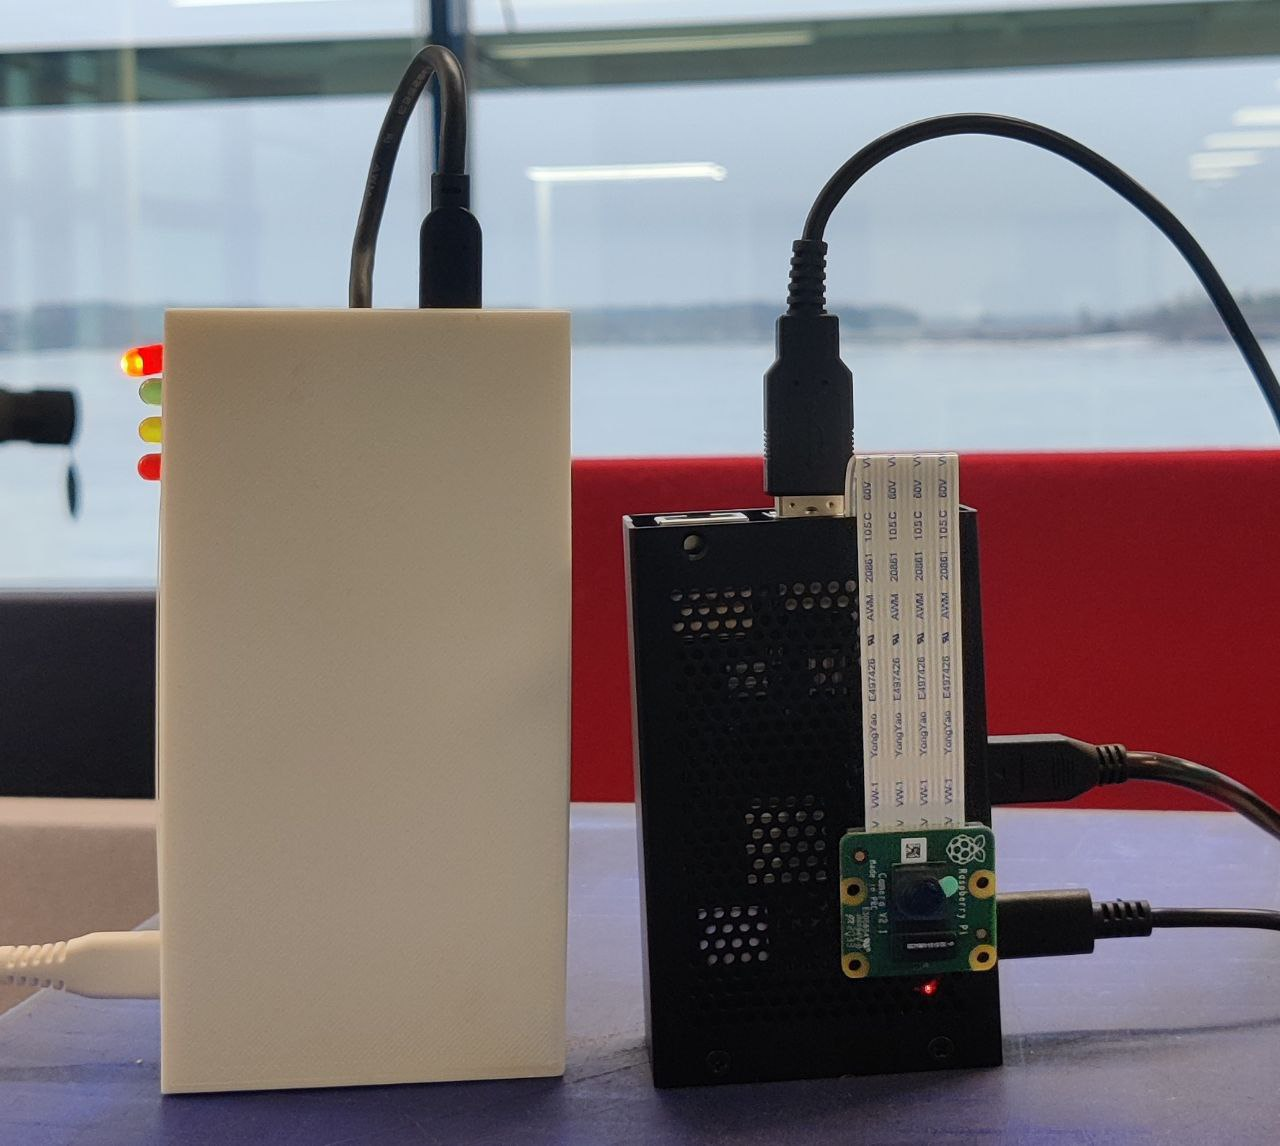
\includegraphics[width=0.5\textwidth]{Master's thesis/images/equipment.jpg} 
    \caption{RADAR and Camera}
    \label{fig:AoA}
  \end{center}
\end{figure}  

\section{Data Pipeline}
\label{section:environments}
For Radar Data
For RGB Data
For PIR Data


\section{Feature Extraction}
\label{section:environments}


